% TikZ architecture diagram for PlenumHub
\documentclass[tikz]{standalone}
\usepackage{tikz}
\usetikzlibrary{shapes, arrows.meta, positioning}
\begin{document}
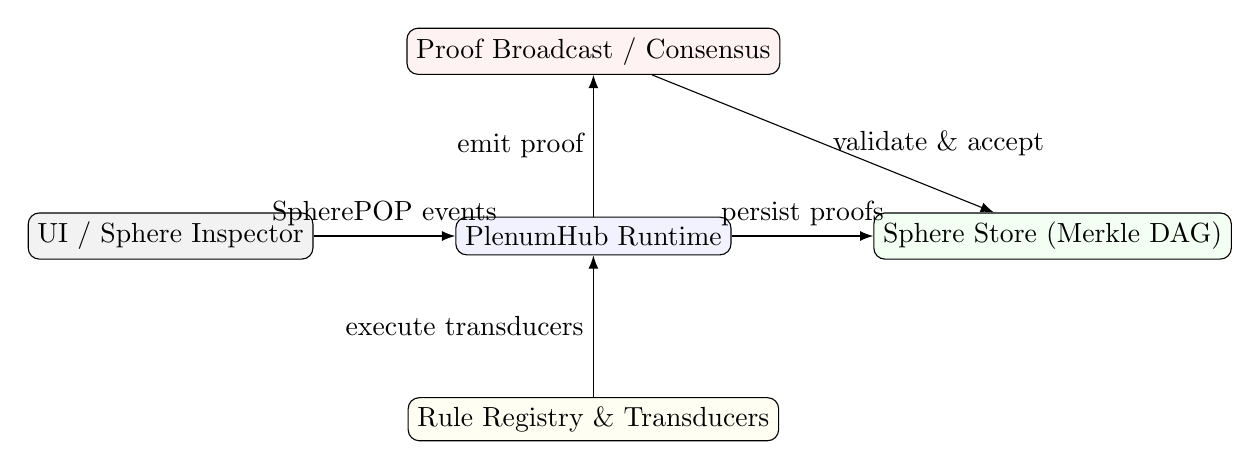
\begin{tikzpicture}[node distance=18mm, auto, >=Latex]
  \node[draw, rounded corners, fill=gray!10] (ui) {UI / Sphere Inspector};
  \node[draw, rounded corners, fill=blue!5, right=of ui] (runtime) {PlenumHub Runtime};
  \node[draw, rounded corners, fill=green!5, right=of runtime] (store) {Sphere Store (Merkle DAG)};
  \node[draw, rounded corners, fill=yellow!5, below=of runtime] (rules) {Rule Registry \& Transducers};
  \node[draw, rounded corners, fill=red!5, above=of runtime] (consensus) {Proof Broadcast / Consensus};
  \draw[->] (ui) -- (runtime) node[midway,above] {SpherePOP events};
  \draw[->] (runtime) -- (store) node[midway,above] {persist proofs};
  \draw[->] (rules) -- (runtime) node[midway,left] {execute transducers};
  \draw[->] (runtime) -- (consensus) node[midway,left] {emit proof};
  \draw[->] (consensus) -- (store) node[midway,right] {validate \& accept};
\end{tikzpicture}
\end{document}
